\chapter{Related work}
\label{chp:related-work}

This chapter is dedicated to a thorough review of past literature in this domain, including both classic and recent works. Section \ref{sec:related-work-areas} presents various research wings in this domain, followed by a detailed discussion on various methods of seed selection in section \ref{sec:related-seed-selection} - a key topic in influence mining. Finally, \ref{sec:related-work-resilience} spotlights works from a different community working on network dismantling; this branch is focused on the opposite dimension of the same phenomenon. Where influence mining aims to identify the best method to \textit{grow} an effect through a set of seed nodes via information diffusion, the objective of network dismantling is to identify the best method to \textit{shrink} or decompose a network. Both ideas are cut from the same fabric - identifying influential nodes.


	\section{Research areas}
	\label{sec:related-work-areas}
	Before moving to the crux of the matter, it is vital to reiterate that the influence mining domain is vast and there have been numerous studies and review conducted on the core idea.
		
		\subsection{On influence maximization}
		Domingos and Richardson \cite{domingos2001} were first to study identification of influential users and influence propagation. They model a social network as Markov Random field (an undirected graph with nodes as random variables and edges as dependencies between variables) and proposed heuristics for selection of most influential users.
		
		Extending Domingos’ work, Kempe et al. \cite{kempe2003} took greedy approximation approach to guarantee influence maximization. They focus on two basic and very frequently used diffusion models: Linear Threshold model and Independent Cascade model. In the LT model, each active neighbour $v\in V$ of an inactive neighbour $u\in V$ of network $G:(V,E)$ exerts some influence on $u$ with some probability weight $w_{v,u}$; the inactive user $u$ chooses a random uniform threshold $\theta_u$ representing minimum collective weightage required for it to be active, if $w_{v,u}\ge \theta_u$, then $u$ gets activated. The IC model says that the chance of each user $v$, which just became active on time step $t$, of influencing its inactive neighbour $u$ is independent of the past history; the probability $p_{v,u}$ is the strength of $v$ to influence $u$. Kempe et al. showed that although influence maximization problem is NP-Hard, the maximization function is submodular and monotone and therefore, we can exploit these properties to get an initial seed nearer than 63\% of the optimal set in linear time. In addition, they discuss some more tuned-up models like Triggering model, in which an inactive user $u$ independently chooses a set of active user in his neighbours that can trigger it to become active; these triggering users are the ones that genuinely can affect $u$, and then Only-Listen-Once model with efficiency within 63\%, i.e. \textit{$(1-\frac{1}{e})$} (where $e$ is the base of natural log, also called exponential constant), in which an inactive user $u$ can be activated only by one of his active neighbours. The Threshold model works on the basis of critical mass actions introduced by Granovetter \cite{granovetter1978} which proposes that an action is adopted by a person if certain number of people (or threshold) have adopted the same action; Cascade model on the other hand, is similar to SIR disease model used in epidemiology \cite{hethcote1989}, and follows the law of diminishing returns \cite{goldenberg2001}. Both of these models use timestamps of user actions; each user is either active or inactive, and the possibility of an inactive user to become active increases when its neighbouring users turn active.
	
		Chen et al. \cite{chen2010} have further extended Kempe et al. – influence maximization problem, simultaneously attacking the scalability issue of simply greedy approximation technique as well as performance lack in heuristic based solutions. %They provide a parameter to tune-up algorithms in their model, MIA (Maximum Influence Arborescence) according to the scale and performance.
		
		Watts et al. \cite{watts2007b} proposed a model called \textit{Big Seed Marketing} that reliably delivers higher marketing gain that may be achieved with any complex viral marketing model or high-budget mass marketing. Their model guarantees that a parameter called reproduction rate, $R=\beta z$ can be achieved greater than 1. Where $\beta$ is defined as the constant probability of word-of-mouth spread and represents the average of number of people that a news is spread to, by individuals.
	
		Leskovek et al. \cite{leskovec2007b} target the influence propagation problem in a different way, calling it Outbreak Detection. The problem is to detect nodes in a network, through which a virus could spread, as quickly as possible. Their work is generalized and they define influence maximization problem to be a special case of it. They developed an efficient algorithm using an approach, lazy-forward optimization\footnote{A programming technique in which instead of executing an inner function fully, a shallow function is called which returns an output from a pre-calculated heap/map.}, to select new seeds; the algorithm is 700 times more efficient than simple Greedy solution.


		\subsection{On learning influence probabilities}
		Since in the influence mining process, active nodes in the network tend to influence other inactive nodes based on certain probability, there is an open branch to identify the right probability instead of an arbitrary number. This is because not all nodes are equally influential, nor are they equally influenced, and neither is each action same in exerting influence. For example, a celebrity talking about a brand of spectacles is likely to attract people who wear spectacles; on the other hand an olympic athlete promoting a crash course on knitting is unlikely to catch as much traction.
		
		Kazumi Saito et al. \cite{saito2008} discussed how to learn influence probabilities from IC model from historical influence propagations. Their work has limitations, when applying to real-World problems, most significant of which is that their model generates initial seeds which might have less, even a single action performed, but due to larger number of neighbours, they end up being very influential nodes.
		
		There is a major outstanding problem with the existing work is that the researchers use some naïve techniques to choose probabilities associated with the edges. Like IC model assumes that the edges have uniform probabilities; WC or weighted cascade model, as proposed by Wei Chen et al. \cite{chen2010} calculate the edge probabilities between any pair of nodes $u,v$ as $p_{v,u}=\frac{1}{d^{-}_{u}}$ where $d^{-}_{u}$ is in-degree of node $u$; Trivalency model chooses a uniform probability between predefined high, medium and low (0.1, 0.01, 0.001). Kazumi Saito et al. \cite{saito2008} initially target this ignored factor by learning influence probabilities in IC model using Likelihood Maximization; they assume that propagation trace is a set of users $V$, activating in discrete time steps, but their assumption that for each inactive user $u\in V$, there must exist an active neighbour $v\in S;S\subset V$ that became active in time step $t_{u}-1$ (here, $t_u$ is the time step when node $u$ was activated), their model is more theoretical than practical. Goyal et al. \cite{goyal2011} address this by implementing different methods of learning influence probabilities using past propagation traces and compared different outcomes of greedy algorithm in IC model with naïve techniques. They divide the dataset into training data for learning influence probabilities and test data for influence maximization.
		
		In a different study \cite{goyal2010}, Goyal et al. included another aspect by showing in their experiments that the influence probabilities decay exponentially as time unfolds. They study the same process under an alternate model, the General Threshold Model. They used this model and made the probabilities decline with time. The assumption behind this is that if a user u performs an action, like tweeting, then his linked user v will either re-tweet shortly after the tweet or never. This decline of probability is observed to be exponential.

		Barbieri et. al. \cite{barbieri2014,martinvcic2017} applied the phenomenon for link prediction; Tang et. al. \cite{tang2015b} use the same for negative link prediction (e.g. dislikes); \cite{mcgee2013} predicted location of users based on their social ties; Chen et. al. in a recent study showed how social influence can be used in music recommendation systems \cite{chen2019}.
		
		\subsection{On community detection}
		Due to the complexity of the problem, some studies suggest taking divide and conquer approach to solve it. Mahmood et al. \cite{mehmood2013} contribute by devising a greedy hierarchical method to partition a social network into communities, each consisting of nodes sharing common behaviour that has been learnt by training data. Their proposed model -- unlike most of the studies -- does not pick these $k$-users (or seed) randomly or based on centrality, etc. but rather, first communities within the network are found out and then in those communities, users with highest centrality are chosen such that the total of all users chosen is $k$. The idea behind comes from an interesting study by Goyal et al. \cite{goyal2009} who articulate that in a network, there exist tribes based on some subject of interest of the members of the tribe and leaders of these tribes that are the most influential people within local tribes. This community-based influence mining has following benefits over centrality-based methods:
		
		\begin{enumerate}
			\item The selection of seed is guaranteed to be from vast area of whole network, instead of a single more coupled region where users are highly interconnected.
			
			\item The highly influential nodes are decided on the basis of attributes of communities, not globally, giving a chance to the nodes that are locally influential but may not be globally influential.
			
			\item Computation time required is divided among communities, thus, even if we use influence maximization process, the time complexity will be reduced drastically.
		\end{enumerate}
	
		The authors proposed GuruMine, a pattern mining approach \cite{goyal2009} for finding out leaders and their tribes in a network where leaders are the users with high influence and tribes are set of users being influenced by leaders over a class of actions. Their framework proposes that given:
		
		\begin{itemize}
			\item A network $G:(V,E)$ of $V$ nodes and $E$ edges.
			
			\item A set of user actions $A$ (also referred to as action log).
			
			\item Threshold parameter $\pi$ denoting maximum propagation time. %TODO: use some other symbol instead of pi
			
			\item Threshold parameter $\psi$ denoting the least value of influence of a user $u$ with respect to an action for at least $\pi$ time.
			
			\item Threshold parameter $Infl_\pi (u,a)$ as minimum influence required by user $u$ performing action $a\in A$ to qualify as leader.
			
			\item Subset $I\subseteq A$ representing a complete set of actions performed by user $u$.
			
			\item $\xi$ be the minimum number of actions required for $u$ to qualify as leader while satisfying $Infl_\pi (u,a)$\footnote{In the original paper, this notation is $\sigma$. It is changed here to avoid confusion with $\sigma$ which is defined as measure of Influence in following chapters of this menuscript.}.
		\end{itemize}
		
		 User $u$ is a leader if $|I|\geq \xi and |Infl_\pi (u,a)|\geq \psi \forall a\in I$. For example, if we choose $\pi$=5 units, $\psi$=3 units, $\sigma$=2 units, then a user $u$ is leader if within a time slot of 5 units, users reachable from $u$ perform at least 2 actions, each action performed at least in 3 time steps. The leaders can then be tribe-leaders, a stronger notion of defining leaders for a class of actions.

		The limitation with community-based approaches is that not every network has community structure or hierarchies, thus rendering divide and conquer inapplicable.		
		
		\subsection{On heterogeneous networks}
		A distinctive work by Liu et al \cite{liu2010} discussed topic-level direct and indirect influence in heterogeneous networks. Their study is divided into: topic distribution modeling and strength estimation; the strength of influence is analyzed by probability $(p_1-p_2)$, where $p_1$ is the probability of a user’s n-degree friends to be induced to perform the same action which he did and $p_2$ is the average probability of whole population to perform that same action.
		
		\subsection{On veracity}
		Some researchers scrutinize veracity of information in social networks. Goldenberg et al. \cite{goldenberg2001} focused word-of-mouth phenomenon for marketing and information propagation and discuss effect of strong and weak ties on the speed of adoptation of an idea or product. Farajtabar et al. \cite{farajtabar2015} recently presented a framework to backtrack historical data in a social network and identify source node of malicious information. Eytan Bakshy et al. \cite{bakshy2011} argued that the word-of-mouth effect is not achieved by a small number of people but a big proportion of them. Janders \cite{jenders2013} worked on distinguishing a viral event from a non-viral event on Twitter. Ma et. al questioned the very idea of popularity, arguing that viewership is a neutral event and is not the right measure of content popularity \cite{ma2013}.

		\subsection{On benchmark methods}
		Benchmarking is one of the areas rarely explored by the researchers. A recent paper by Arora et. al. \cite{arora2017} is an open critique on the influence maximization studies. This paper evaluates several algorithms using vibrant benchmarking techniques focusing on time and memory efficiency, quality and scalability of each method. The authors establish that the efficient methods miss out on quality, the ones which offer quality cannot be scaled, and that the best methods for practical cases are the ones with higher quality and time efficiency. Moreover, some of the methods presented do not guarantee approximation on both LT and IC models.
		
		
	\section{Scalability problem and seed selection heuristics}
	\label{sec:related-seed-selection}
	In attempts to find workaround for inherent scalability problems when maximizing influence in large networks, several studies proposed different heuristics to select influential nodes. A classic and comprehensive article on centrality by Freeman \cite{freeman1979} provides foundation for various heuristics to come. Goyal et al. \cite{goyal2012} presented a greedy method to select initial seed nodes such that the coverage is at least up to a given threshold in logarithmic time, while approximation guarantees are similar to that of original greedy algorithm (see \ref{alg:influence-greedy-solution}). Encountering the scalability problem again on large networks, the research community has produced heuristics and algorithms in abundance to select seed nodes:
	
		\subsection{Topological methods}
		The term \textit{topology} refers to the structural position of nodes in the graph. These methods exploit the topological value of nodes rather than sampling or simulations. A node, which lies in the core of graph tends to be highly influential as compared to the nodes which lie in the boundaries or outermost area. While the key benefit of these is their efficiency, their major drawback is lack of theoretical guarantee on quality. There are several topological methods, and different variations out of which, some are given here.
		
		\begin{enumerate}
			\item Degree Centrality: a measure of how many connections a user has. k-users with the highest degree centrality are selected with an expense of $O(|V|)$ complexity.
			
			\item Closeness: the inverse of the average length of the shortest paths of a user to all other user; closeness value is always between 0 and 1. Users with the highest closeness are selected with an expense of $O(|V|)$ complexity.
			
			\item Betweenness: a measure of shortest paths on which it exists. k-users with the highest betweenness are selected with an expense of $O(|V|)$ complexity by using a faster solution to calculate betweenness by Brandes \cite{brandes2001}.
			
			\item Eigenvector centrality \cite{bonacich1987}: a measure of influence of a user in the network by assigning relative score to a user based on the concept that connections to high-scoring users contribute more to the score of the user; this value is always between 0 and 1. k-users with the highest Eigen value are selected with an expense of $O(|V|)$ complexity.
			
			\item Subgraph centrality: measures the weighted sum of walks of various lengths from and to the node under observation \cite{estrada2005}. However, the conjecture from the authors that \textit{if a graph has identical subgraph centrality for all nodes, then the closeness and betweenness centralities are also identical for all nodes} has been disproven by \cite{stevanovic2013}.
			
			%\item No-neighbours: this method selects only the highest degree users that are not directly connected to each other to ensure that we do not have users of a specific section of the network; the additional cost is $O(\frac{k^2}{2})$.
			
			\item Coreness: a measure to describe network cohesiveness. A network $H$ is $k$-core if it is connected maximal subnetwork of original network $G$ and the degree of each node is at least $k$. Coreness of each node in $H$ is defined as $k$. The additional cost of this method is $O(|V|)$ by using algorithm proposed by Batagelj et al. \cite{batagelj2003}.
			
			\item Centrality in Community: a cluster of users - a sub-graph, which are highly connected with each other but loosely connected to users in other communities. Users are selected from each communities with highest centrality, such that their sum is equal to k. Discovering communities by calculating the leading non-negative Eigen-vector of sub-graphs \cite{newman2006b} has an additional cost of $O(|E|+|V|^2)$. There are other community detection algorithms which can be applied to extend this technique.
			
		\end{enumerate}
		
		\subsection{Simulation based Algorithms}
		These methods perform Monte Carlo simulations to discover influential nodes in iterative manner. They provide guarantees of effectiveness within certain approximation of the best possible solution, but often fail to scale on large data sets due to the time and space complexity.
		
		% Refer to Debunking the Myths of Influence Maximization: An In-Depth Benchmarking Study
		\begin{enumerate}
			\item Greedy: exploiting the monotone and sub-modular property of the influence maximization problem, a Hill climbing greedy based algorithm has been proposed by \cite{kempe2003}, which guarantees a solution within approximately 67\% of the optimal solution.
			
			\item CELF: these are extensions of the original Greedy algorithm, with same worst time complexity, but their average time complexity is up to 27 times better than the predecessor. CELF algorithm \cite{leskovec2007b} takes a lazy-forwarding approach and instead of recomputing the influence spread of every node in each iteration, it exploits the sub-modularity property and thus reuses the pre-computed marginal gain of individual nodes in each iteration during simulation.
			
			\item CELF++: \cite{goyal2011b} further optimizes the idea behind CELF and increases the efficiency by up to 55\%. This algorithm maintains a heap $Q$ such that it preserves not only the marginal gain of individual node, but also the marginal gain of each node coupled with the best node identified in prior iteration. These values are reused during the simulation to further reduce the redundant computation of influence spread.
		\end{enumerate}
		
		\subsection{Sampling Algorithms}
		\begin{enumerate}
			\item Adaptive Sampling: a variant of sampling technique presented by Lipton \cite{lipton1989}. In an iterative way, the nodes in a network are ordered by a metric (e.g. Degree centrality) and top node or a batch of nodes are removed from the network and the process is repeated on the largest connected component until the network is completely dismantled. The same technique was used for Betweenness centrality in \cite{hussain2019} for better results than Degree centrality, proving that this technique can be used as an extension of any topology-based method. 
			
			\item TIM: draws $\theta$ number samples of reverse reachable (RR) sets from a directed network. Its results outperform the then state-of-art on largest networks tested in the literature by an near optimal efficiency of $(1-\frac{1}{e}-\epsilon)$, while offering time complexity of $O((k+l).(n+m).log(\frac{n}{\epsilon^2}))$ \cite{tang2014}. The idea behind TIM is that a node $u$ is influential if it frequently appears in the samples such that it has direct edge from each node $v$ in RR samples. %TODO: Define epsilon here
			
			\item IMM: \cite{tang2015} adds statistical optimizations to TIM in estimation and improves accuracy by adding little complexity. These techniques however, have been demonstrated only on IC model. However, these results were challenged by \cite{chen2018}, but the challenging paper also suggests workarounds with minor addition to time complexity to achieve the promised results.
			
			\item StaticGreedy: fixes a long-standing issue of Hill climbing approach that it needed many MC simulations to guarantee approximation \cite{cheng2013}. This algorithm employs a simple and effective technique of MC snapshots, i.e. instead of dynamically creating snapshots during the spread simulation, a collection of network snapshot is created and all simulations are run only on that set. Thus avoiding the need for reconstructing snapshot networks as well as guarantee the accuracy on limited number of MC simulations.
			
			\item PMC: \cite{ohsaka2014} furthers the StaticGreedy on even larger networks through graph pruning, requiring even lower number of snapshots than the former. For each randomly generated graph for MC simulations, a strongly connected weighted DAC (Directed Acyclic Graph) is computed, where the weight on nodes denote the number of nodes reachable. The influence $\sigma$ is then computed for each node via averaging gain in each DAC through BFS (Breadth First Search).
			
		\end{enumerate}
		
		\subsection{Community focused Variant}
		The topological and heuristic methods used on smaller communities identified by community detection algorithms take divide and conquer approach by splitting a large graph into communities and computing influential nodes within these communities. The most notable work in this area is by Wang et. al. \cite{wang2010}, which proposed CGA-Community based greedy algorithm which detects communities in a social network through dynamic programming and uses MixedGreedy algorithm \cite{chen2009} for influence maximization simulation within these communities. He et. al. \cite{he2015} furthered the idea later by first identifying \textit{super nodes} (strongly connected communities) and then choosing one spreader node from each super node. This method improves on time complexity as well as simulates realistic community detection.
		
		The community focused variant has a pitfall that it can work only on the networks which have community structure, Social networks are best examples here. However, on sparse networks, this technique is not applicable.
		
		\subsection{Scoring Algorithms}
		This class of algorithm assigns a particular rank or score to each node and selects $k$ nodes with highest scores as seed set. Such methods are quite effective when used on particularly friendly types of networks for which their baseline technique was tailor made.
		
		\begin{enumerate}
			\item Pagerank: Brin and Page made a breakthrough in the web search engine history in 1999 \cite{pagerank1999} with their proposed web page ranking method. A web page gets higher rank if it is linked with more web pages. The same idea is applied on networks to identify influential seed nodes. If $u$ is a node to be ranked and $v\in N_u$ are all nodes directly with $u$, then the rank $R_u=c\sum_{v\in N_u}\frac{R(v)}{|N_v|}$. The algorithm is very fast with $O(|V|+2|E|)$ time complexity.
			
			\item Collective Influence: Morone et. al. \cite{morone2015} discovered that on larger networks, influential nodes are often weakly connected, and that the same influence spread can be achieved with a much smaller seed set than the other heuristics suggest. Collective influence is calculated by multiplying the degree of node $u$ with sum of all degrees of the set of its neighbouring nodes $N_u$ up to some distance $\delta$ (e.g. $\delta=1$ represents direct neighbours, $\delta=2$ represents neighbours of direct neighbours and so on). Therefore if $\Lambda_u$ denotes set of all nodes of $u$ within a distance $\delta$, then simply, $CI(u)=d_u * \sum d_{\Lambda_u}$. The running time complexity of this methods is $O(|E||V|log|V|)$.
			
			\item SIMPATH: competes directly with LDAG \cite{chen2010b} and presents the phenomenon that in LT model, the spread of a node is driven by the spread of the induced subgraph consisting of its neighbours. Mathematically, $\sigma(S)=\sum_{u\in S}\sigma(u\cup (V-S))$. This optimization significantly reduces the estimation calls. Consequently, a score is assigned to each node by summing up the probabilities all simple paths from $u$ to other nodes. The length of the simple paths are restricted through a tolerance parameter $\eta$, as computing full length paths itself is NP-hard, and useless because of the property of diminishing returns.
			
			\item EaSyIM: \cite{galhotra2016} is the state of art in the class for its low memory footprint of $O(|V|)$ and linear time complexity of $O(kD(|V|+|E|))$ where $k$ is the size of seed set and $D$ is diameter of network. The algorithm assigns EaSyIM score to each node by calculating weighted sum of number of paths of length $l$ starting from $u$, while the weight of path is the product of edge probabilities that lie on that path.
			
			\item IMRank: is a rank refinement technique on top of other scoring algorithms for IC model \cite{cheng2014b}. A scoring method is used to calculate scores in first iteration, but in the consequent steps a last-to-first reverse rank ordering method is used to improve the efficiency of marginal gain estimation. This algorithm guarantees the self-consistent ranking by calculating marginal ranking of nodes in iterations with respect to their previous rank.
			
		\end{enumerate}


	\section{Network dismantling and Resilience}
	\label{sec:related-work-resilience}
	This problem is conventionally presented as graph dismantling, which is to identify a minimal set of vertices such that removing this set disintegrates the original graph into connected sub-graphs of sizes no larger than predefined. Formally, a connected graph $G=(V,E)$ is decomposed by removing the edges in iterative manner such that there does not remain any sub-graph $H_i$ for which there exists an edge between any pair of nodes $i,j$.

		\subsection{Resilience}
		\label{subsec:related-work-resilience}
		Resilience, as described in \ref{sec:domain-resilience} is a network's ability to hold itself together when its nodes are individually under a targeted attack. The more resilient a network is, the more nodes will have to be taken down in order to dismantle the network. Latif et al. \cite{latif2014} studied network resilience under different kind of networks, their work focuses on exploiting the structure of different networks like scale-free and small-world networks and compare the resilience of these networks under different forms of attacks.
		
		Among the most basic methods are degree and other centrality based. Degree centrality is generally used alongside Random selection method for benchmarking and comparison purpose. \cite{braunstein2016} shows that Eigenvalue centrality stands out on Erdos–Rényi random graphs among other centrality heuristics while introducing their Min-Sum decycling algorithm.
		
		Apart from centrality based methods, Pagerank \cite{pagerank1999} stands out as a fast and effective baseline heuristic to identify resilient nodes. Lü et. al \cite{lu2011} introduced LeaderRank, an algorithm based on Random walk which outperformed Pagerank on directed social networks.
		
		Chen \cite{chen2012b} and others proposed a \textit{local centrality} method, which computes the centrality as sum of degrees of 2-step neighbourhood of a node \ref{eq:local-centrality}:
		
		\begin{equation}
			\label{eq:local-centrality}
			C(v)=\sum_{u\in\Gamma(v)}(\sum_{\omega\in\Gamma(u)}N(\omega))
		\end{equation}
		
		Where $\Gamma(u)$ is the set of neighbouring nodes of $u$ and $N(\omega)$ is the set of nieghbouring nodes to second degree (neighbours of neighbours). This method provides a good trade off between effectiveness which centrality based methods miss, and expensive computation time like Greedy solution.
		
		Among the most established topological methods, $k$-shell decomposition algorithm was first presented in a classic study \cite{seidman1983}. Analogous to atomic structure, the most central nodes are in the $k_{max}$ shell, then the rest of the nodes belong to one of the shells between $k_1$ and $k_{max-1}$. The nodes in $k_1$ shell are those with degree = 1. In order to identify $k_n$ shell, all the nodes with degree $n-1$ are removed in iterative manner. The $k$-shell decomposition seems to overlap with $k$-core. However the key difference is that a graph's $k$-core is the maximal subgraph in which each node has a degree $k$ or higher. On the other hand, $k$-shell is a set of nodes which are part of the subgraph $k$-core but not $(k+1)$-core. The $k$-shell methodology was used in the context of internet resilience by Carmi et. al. \cite{carmi2007} who studied the Internet map and showed that using their proposed enhancement, the Internet map can be decomposed in 6-shell decomposition.
		
		Later, Kitstak \cite{kitsak2010} propagated this method on large scale on Social networks, including one with 3.4M nodes under SIS\footnote{Susceptible-Infected-Susceptible} and SIR\footnote{Susceptible-Infected-Recovered} models of epidemiology. Their study confirms the hypothesis that it is the topology, not the connectedness of a node which decides how vital it is in the network when spreading a contagion.
		
		An argument can be made against k-shell decomposition method that it has a limitation particularly in Social networks. For example, \cite{borge2012} found out that for rumor diffusion, k-shell method is not very effective. We argue that the said method identifies the \textit{oldest} nodes as influential, while in social networks are organically built, the network takes community form and diverges into Leaders and Tribes, as shown by Goyal et. al. \cite{goyal2008}.
		

	\section{State-of-art}
	\label{sec:related-work-state-of-art}
	Among the recent work in the domain of influence mining, one of the most prominent works is by Lei \cite{lei2015}. It presents a framework of influence maximization in online mode, which has the capability of switching between Exploit mode when exact information about influence probabilities is available, and Explore mode when it the probabilities are to be calculated. The proposed model is incremental, and reuses the users’ feedback information extracted from previous iterations. Traditionally, influence maximization problems have an offline setting, in which the network is fixed and edge probabilities are known. The author redefines the problem as a weighted graph $G=(V,E,p)$ where probabilities $p_{u,v}$ (probability of node $u$ to influence node $v$) are not known; the objective is to find a seed set $S$ with $|S_n|\leq k$, which maximizes the set of edges $E[|\cup_{1\leq n \leq N}I(S_n)|]$ where $k$ is the budget consisting of $N$ trials with $1\leq k\leq |V|$, $I(S_n)$ is the set of nodes influenced in trial $n$.
	
	On community detection in networks, Fortunato \cite{fortunato2016} attack a long-open problem that there is no universally accepted protocol about defining goodness of a community detection method. The author defines three classes to assess performance of a community detection method:
	
	\begin{enumerate}
		\item Internal Connectedness: this class defines how cohisive the graph is. This measurement is calculated from three variables:
		
		\begin{itemize}
			\item Internal Degree ($k^{int}_{C}=\sum_{i,j\in C}A_{i,j}$) is sum of internal degrees of all nodes in a subgraph $C$ in the graph adjacency matrix $A$.
			
			\item Average Internal Degree ($k^{avg-int}_{C}=\frac{k^{int}_{C}}{n_C}$) is the sum of average internal degrees in $C$.
			
			\item Internal Edge Density ($\delta^{int}_{C}=\frac{k^{int}_{C}}{n_C(n_C-1)}$) is the ratio between number of internal edges and number of possible internal edges in $C$.
		\end{itemize}
		
		\item External Connectedness: in contrast to internal connectedness, this class defines how embedded the network between sub-networks. There are three main variables to check the external connectedness:
		
		\begin{itemize}
			\item External Degree ($k^{ext}_{C}=\sum_{i,j\not\in C}A_{i,j}$) is sum of external degrees of all nodes in a subgraph $C$.
			
			\item Average External Degree ($k^{avg-ext}_{C}=\frac{k^{ext}_{C}}{n_C}$) is the sum of average external degrees in $C$.
			
			\item External Edge Density ($\delta^{ext}_{C}=\frac{k^{ext}_{C}}{n_C(n-n_C)}$) is the ratio between number of external edges and number of possible external edges in $C$.
		\end{itemize}
		
		\item Hybrid Measure: this class can have plenty of examples, like:
		
		\begin{itemize}
			\item Total Degree, or Volume ($k_C=\sum_{i\in C,j}A_{i,j}$) is the sum of all degrees.
			
			\item Average Degree ($k^{avg}_{C}=\frac{k_C}{n_C}$) is the average degree of all nodes.
			
			\item Conductance ($C_c=\frac{k^{ext}_C}{k_C}$) is the ratio between external degree and total degree of $C$.
		\end{itemize}
		
	\end{enumerate}
	
	The author iterates that modern view of community detection is more probabilistic than classical view, which considers counts. In modern view, a \textit{strong community} is the one in which the nodes in a subgraph has higher link-probability than external nodes. Where in a \textit{weak community}, average link probability within a subgraph exceeds the average link-probability of nodes in the subgraph with nodes of any other group.
	
	Lü, et al. \cite{lu2011} present an empirical, yet comprehensive article on vital nodes in a network and means to extract them. Key contribution in this paper is the way several classes of vital node extraction are discussed:
	
	\begin{enumerate}
		\item Structural Centralities: this class of centralities takes into account the structural properties of nodes. Authors further categorize this class into two subclasses: Neighbourhood-based and Path-based centralities.
		
		\item Iterative Refinement Centralities: in this class, the importance of a node is determined by the importance of neighbours, iteratively. Authors discuss several methods for undirected networks like Eigenvector centrality, and directed networks like PageRank.
		
		\item Node Operation: contrary to using structural properties, this class deals with identifying targeted nodes in a network, which could be attack-sensitive with respect to connectivity, stability, or node contraction, etc.
		
		\item Dynamics-sensitivity: here, some context about the network is introduced, like time stamp. Social networks, for example, are evolving, and their dynamics are important when identifying vital nodes.
		
		\item Influence Maximization Methods: the NP-hard problem of identifying an optimal vital set of nodes in a network. There are various aspect of this problem, for example, finding out minimal set of optimal nodes; identifying a set of optimal nodes with a fixed budget; finding a set of nodes with fixed desired influence. This class is quite broad and is further broken into Structural and Functional Influence Maximization.
		
		\item Greedy Method and Heuristics: these are the most commonly observed classes, proposed as a scalable alternative to IM. Greedy method has complexity of $O(n^2)$ and guarantees accuracy within a factor $1-\frac{1}{e}\approx 0.63$ of optimal results.
	\end{enumerate}
	
	The above methods are discussed on unweighted, weighted and bipartite networks for their performance.
	
	In the area of network resilience, a notable series of experiments were conducted to further the state-of-art. Gao \cite{gao2016} et al. have studied resilience in complex networks and proposed a general analytical framework, which provides a one-dimensional view for multi-dimensional complex networks. This paper does not introduce a specific algorithm, but rather guidelines on how to design methods to depict resilience within a real-world network. 
	
	On rank-based methods, Morone, Makse and others \cite{morone2015} rejuvenate the state of art using Percolation\footnote{a classical theory which studies the interaction of particles in a random medium\cite{shante1971}}. The authors proposed optimal percolation method which determines the minimum seed set required for a structural collapse. The influential nodes are identified by calculating a Collective Influence rank with respect to certain radius $l$, i.e. $CI_l(u)=(k_u-1)\sum_{v\in H(u,l)}(k_v-1)$, where $u$ is the node whose CI rank is being calculated, $H(u,l)$ is subset of the network $G$ which includes all neighbouring nodes within the radius $l$ from node $u$. In the experiments on random graphs, CI outperform other rank-based methods (High-degree Adaptive, Pagerank and k-shell decomposition) as well as topological methods. \cite{pei2018} recently discusses the performance of this method thoroughly on brain networks. However, CI is still computationally expensive when scanning for larger radii; on the other hand, it produces far from optimal results for smaller values of $l$ (see \cite{clusella2016}).
	
	Factoring in the time complexity, Mugisha et. al. recently proposed Belief Propagation-guided Decimation (BPD) \cite{mugisha2016}. This method computes a probability for each node via the equation \ref{eq:bpd}.
	
	\begin{equation}
		\label{eq:bpd}
		q_i^0 = \frac{1}{1+e^x \left[1+\sum\limits_{k\in N_i(t)} \frac{1-q_{k\rightarrow i}^0}{q_{k\rightarrow i}^0 + q_{k\rightarrow i}^k} \right] \prod\limits_{j\in N_i(t)} [q_{j\rightarrow i}^0 + q_{j\rightarrow i}^j]}
	\end{equation}
	
	In this formula, $q_i^0$ is the suitability of node $i$ for removal as probability between 0 and 1; $N_i(t)$ denotes set of neighbour nodes of $i$ in time step $t$ where $i$ can pass a message; the probability $q_{j\rightarrow i}^0$ represents suitability of node $j$ for removal if $i$ has already been deleted prior to it; $q_{j\rightarrow i}^j$ is the probability that node $j$ is suitable as root node given that $i$ has been removed.
	
	The experiments performed on Random and Scale free networks and compare BPD specifically with CI and show that BPD not only outperforms CI in execution time, but also in efficiency given that the parameter $l$ is kept low for CI. However it is important to observe that BPD tends to start decomposition process slowly and exhibits a sharp drop, therefore the decomposition process has to be executed completely for it to perform correctly. This behaviour is depicted in Figure \ref{fig:bpd-ci-comparison}.
	
	\begin{figure}[h]
		\centering
		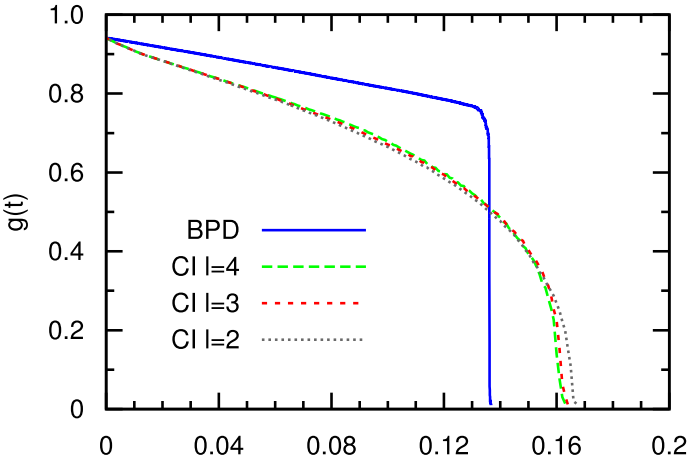
\includegraphics[width=0.7\textwidth]{bpd-ci-comparison}
		\caption[Comparison of Belief Propagation Decimation and Collective Influence]{Comparison of BPD with CI algorithm. On x-axis is the normalized time step and on y-axis is the largest component remaining in the network at time $t$.}
		\label{fig:bpd-ci-comparison}
	\end{figure}
	
	\cite{zdeborova2016} recently extended k-shell decomposition approach with simple fine-tuning. Their algorithm first finds 2-core network and removes the node with highest degree in this network in iterative fashion. This algorithm is named CoreHD, and the results exhibit that it outperforms the CI by a small margin, while significantly reducing the network dismantling time. This method however, focuses more on dismantling and decycling the network faster rather than finding influential nodes. It has not yet been tested under influence spread mechanism.
	
	Overall, BPD is the most efficient; CoreHD has best execution time, while CI is more generic and scalable due to its liberal $l$ parameter.


	\section{Summary}
	\label{sec:related-work-summary}
		
	There are plenty of studies on influence mining and its sub-topics; here is a brief summary of these. The problem of influence maximization, first defined by \cite{kempe2003} was generalized by \cite{leskovec2007b}. A few variations of the same problems were studied by researchers like \cite{goyal2011,morone2015} to view it in dimensions other than conventional network heuristics. The following list summarizes different groups of studies in the domain with prominent works:
	
	\begin{itemize}
		\item On algorithm Optimizations: Great many studies target scalability and efficiency problem on large networks \cite{chen2009,tang2009,chen2010b,goyal2011b,goyal2012,chen2012,jung2012}.
		
		\item Some of the key studies focused on learning influence probabilities for LT, IC and other models, including both classic \cite{granovetter1978} and recent \cite{saito2008,goyal2010}.
		
		\item On identifying Influence: Gladwell thoroughly explained social attributes of influential people in his book \cite{gladwell2006}; \cite{mcpherson2001} define homophily in social networks. On the other hand, Singla et al. prove the existence of correlation phenomenon \cite{singla2008}, while Anagnostopoulos separate influence from homophily and other sources of correlation \cite{anagnostopoulos2008}. On the same idea, \cite{aral2009,lafond2010} later performed randomization tests to distinguish influence from homophily.
		
		\item On Viral Marketing: Studies like \cite{mahajan1990,domingos2001,goldenberg2001,richardson2002,domingos2005,hill2006,leskovec2007,watts2007b,wortman2008,hu2014,barbieri2014} focus on its application in viral marketing, which is clearly a target real-world problem for influence mining \cite{jurvetson2000}.
		
		\item On applications in Social Networks: A cohort of researchers have focused primarily on social networks \cite{borodin2010,ienco2010,bakshy2011,li2013} by examining links between friends and their activities.
		
		\item On Diffusion: the term describing phenomenon of information propagation, has been consistently discussed by many researchers, like \cite{gruhl2004,song2006,song2007,watts2007,anagnostopoulos2008,crandall2008,cha2009,xiang2010,rodriguez2010,rodriguez2011,romero2011,myers2012,li2013,cheng2014,farajtabar2015}.
		
		\item On Veracity: One of the major problems in studying influence in social networks is accuracy of information. \cite{goldenberg2001,guha2004,ziegler2005,golbeck2006,taherian2008,castillo2011,chen2011,holthoefer2012,morone2015,farajtabar2015} attack this critical issue. Lyons showed how serious the information reliability can become in certain applications \cite{lyons2011}.
		
		\item On Context awareness: Some researchers involve context awareness to the problem, rather than core network properties. For example, Haveliwala \cite{haveliwala2002} apply topical detail on PageRank algorithm, while \cite{liu2010,weng2010,li2012} discuss topic-level influence mining. \cite{carnes2007,bakshy2009,bohn2011,barbieri2014} include user content in their studies.
		
		\item On Community detection: A whole different sub-topic of influence mining is community detection. This area is explored by \cite{goyal2008,goyal2009,leskovec2012,mehmood2013,sallaberry2013} and many others.
		
		\item On Resilience: \cite{seidman1983,pagerank1999} build the research foundations. \cite{carmi2007,kitsak2010} scaled the problem on large networks. Studies like \cite{goyal2008,borge2012} talk about resilience purely in context of social networks; Mugisha \cite{mugisha2016} connected resilience with probability learning concept; \cite{zdeborova2016} improved the original k-shell decomposition method; \cite{braunstein2016} showed that Eigenvector centrality outperforms other topological methods on Erdos–Rényi graphs in resilience; \cite{morone2015} proposed a state-of-art ranking method which ranks nodes by computing collective influence of its neighbours.
		
		\item Other heuristics: Since influence maximization is a hard problem, several heuristics have emerged to escape the scalability issue of IM. Starting from classic studies \cite{freeman1979,valente1995}, various heuristics have been presented, for example \cite{kempe2005,kitsak2010,chen2011,aral2011,borgs2014,morone2015,tang2015}.
	\end{itemize}

Recent works in influence maximization focuses mostly on identifying influence, how it propagates in a network in both direct and indirect ways, techniques to maximize influence and learning influence probabilities using past action logs (or transaction logs) of nodes and optimizing existing algorithms for huge networks. In most of the cases, researchers initiate the influence computation from nodes selected randomly, or based on a measure. Such methods are effective in some cases, however they can also lead to problems like selection of nodes from a specific portion of network, more iterations to cover whole network, and choosing less-influential nodes. While there has been high focus on exploiting network properties of nodes for influence maximization, researchers have also attempted to explore content alongside network properties. On one hand, inclusion of content and metadata during analysis boosts the accuracy of the models, but the demerit of such approach is that the models produced are bespoke, they can only work on certain data sets for which they were built.

Albiet all the work reviewed, we have learned that the influence maximization problem is still wide open and its applications growing with time. In the next chapter, we will look at the problem from theoretical perspective in order to affirm that this problem is indeed computationally challenging.

%TODO: add a table to highlight the major challenges in the state of art methods
